
                \begin{figure}
                    \centering
                    \begin{tikzpicture}
                        \pgfplotsset{%
                            width=1\textwidth,
                            height=0.4\textheight
                        }
                        \begin{axis}[
                            xlabel={Start temperature},
                            ylabel={Average dynamic energy (watt)},
                            ymin=0,ymax=100,
                        ]
                        
                        \end{axis}
                    \end{tikzpicture} 
                \caption{A graph illustrating the energy consumption of Cores for test case TestCaseIdle with regards to the temperature of the DUT, experiment \#2, (without outliers)} \label{fig:TestCaseIdle_Cores_temperature_exp2}
                \end{figure}
                